%%
%% 2May2008.tex
%% 
%% Made by Alex Nelson
%% Login   <alex@tomato>
%% 
%% Started on  Sun Dec 21 15:06:27 2008 Alex Nelson
%% Last update Sun Dec 21 15:06:27 2008 Alex Nelson
%%

\begin{figure}[ht]
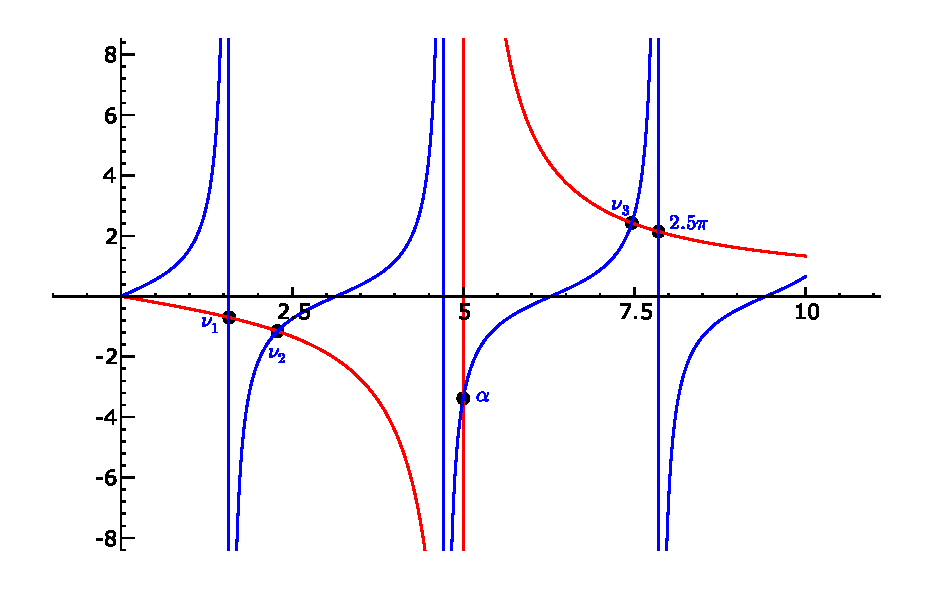
\includegraphics[width=\textwidth]{img/2May2008img1.eps}
\caption[Eigenvalue Relations for Heat Equation]{A Plot of
  the Eigenvalue relations for the Heat Equation from Eq
  \eqref{eqn:2May2008:eigenvalueRelationship} setting
  $\alpha=5$ and $L=1$. The blue line is $\tan(\nu L)$, the
  red line is $2\alpha\nu/(\nu^2-\alpha^2)$. Note that the
  points labeled $\alpha$ and $2.5\pi$ are not eigenvalues
  but singular points of $2\alpha\nu/(\nu^2-\alpha^2)$ and
  $\tan(\nu L)$ respectively that coincidentally overlap in
  the graph program.}\label{fig:2May2008:eigenPlot}
\end{figure}

We were looking at the Sturm-Liouville problem which came
from the heat equation
\begin{equation}
X''(x)+\nu^{2}X(x) = 0
\end{equation}
with the boundary conditions
\begin{subequations}
\begin{align}
X'(0) &= \alpha X(0)\\
X'(L) &= -\alpha X(L)
\end{align}
\end{subequations}
With eigenfunctions $\{\nu\cos(\nu x) + \alpha\sin(\nu x)\}$
where the eigenvalues $\nu^2$ are determined by
\begin{equation}\label{eqn:2May2008:eigenvalueRelationship}
\tan(\nu L) = \frac{2\alpha\nu}{\nu^2-\alpha^2}
\end{equation}
But this isn't the most convenient way to determine the
eigenvalues, as it's not really convenient to do
analytically. The plot of the left hand side in blue and the
right hand side in red is given in figure
\eqref{fig:2May2008:eigenPlot}. We find that
$0<\nu_1<\nu_2<\cdots$. We can normalize the eigenfunctions
$\phi_{\nu}(x)$ to find
\begin{subequations}
\begin{align}
\|\phi_{\nu}\|^{2} &= \int^{L}_{0} (\nu\cos(\nu x)+\alpha\sin(\nu x))^2dx\\
&=\int^{L}_{0} \nu^{2}\cos^{2}(\nu x) + 2\alpha\nu\sin(\nu x)\cos(\nu x) + \alpha^{2}\sin^{2}(\nu x)dx
\end{align}
\end{subequations}
Remember from basic trigonometry
\begin{align*}
\cos^{2}\theta &= \frac{1}{2}(1 + \cos(2\theta))\\
\sin^{2}\theta &= \frac{1}{2}(1 - \cos(2\theta))
\end{align*}
so plugging this in we find
\begin{subequations}
\begin{align}
\|\phi_{\nu}(x)\|^{2} &=
\frac{\nu^2}{2}\int^{L}_{0}(1+\cos(2\nu x))dx +2\alpha\int^{L}_{0}\sin(\nu x)d\left(\sin(\nu x)\right) +\frac{\alpha^2}{2}\int^{L}_{0}(1-\cos(\nu x))dx\\
&=\left(\frac{\nu^2+\alpha^2}{2}\right)L+\alpha\sin^{2}(\nu L)+\int^{L}_{0}\frac{\nu}{2}\cos(2\nu x)-\frac{\alpha^2}{2}\cos(2\nu x)dx\\
&=\left(\frac{\nu^2+\alpha^2}{2}\right)L+\alpha\sin^{2}(\nu L)+\left(\frac{\nu^2-\alpha^2}{4\nu}\right)\sin(2\nu L)
\end{align}
\end{subequations}
We can now take advantage of our eigenrelations
\begin{equation}
\tan(\nu L) = \frac{2\alpha\nu}{\nu^2 - \alpha^2}
\end{equation}
to reduce our calculation of the norm of $\phi_{\nu}(x)$ to
be
\begin{equation}
\frac{1}{2}\left(\frac{\nu^2-\alpha^2}{2\nu}\right) =
\frac{1}{2}\frac{1}{\tan(\nu L)} = \frac{1}{2}\frac{\cos(\nu
  L)}{\sin(\nu L)}
\end{equation}
thus
\begin{subequations}
\begin{align}
\frac{\nu^2-\alpha^2}{2(2\nu)}\sin(\nu L) &=
\frac{1}{2}\cot(\nu L)2\sin(\nu L)\cos(\nu L)\\
&=\alpha\cos^{2}(\nu L)
\end{align}
\end{subequations}
So $\|\phi_{\nu}(x)\|^2 = [(1+L/2)\alpha^2 +
  \nu^2L/2]^{1/2}$, and the orthonormal basis formed for
$L^{2}(0,L)$ satisfies the problem 
\begin{equation}
\partial_{t}u(x,t) = k\partial_{x}^{2}u(x,t)
\end{equation}
where
\begin{equation}
u_{n}(x,t) = c_{n} e^{-\nu^{2}_{n}kt}\phi_{n}(x)
\end{equation}
We need to now find what all the $c_{n}$'s are. (Yes, our
work never ends; we're like Pinkerton's, we never rest.)

To do so, we let
\begin{subequations}
\begin{align}
u(x,t) &= \sum^{\infty}_{n=1}u_{n}(x,t) = \sum^{\infty}_{n=1}c_{n}e^{-\nu^{2}_{n}kt}\phi_{n}(x)\\
u(x,0)&=f(x)=\sum^{\infty}_{n=1}\<f,\phi_n\>\phi_n\\
&=\sum^{\infty}_{n=1}u_{n}(x,0)=\sum^{\infty}_{n=1}c_{n}\phi_{n}
\end{align}
\end{subequations}
Take the difference, we find
\begin{equation}
\sum^{\infty}_{n=1}(c_{n}-\<f,\phi_n\>)\phi_n=0
\end{equation}
because $\phi_n$ is a basis and this linear combination is
zero, we conclude that
\begin{equation}
c_{n} = \<f,\phi_n\>.
\end{equation}

\marginpar{Change boundary conditions}Lets change the
boundary conditions a bit to be
\begin{equation}
X''(x) + \nu^{2}X(x)=0,\qquad X(0)=X(L)=0
\end{equation}
This corresponds to the heat equation
\begin{equation}
\partial_{t}u(x,t) = k\partial^{2}_{x}u(x,t),\qquad
u(0,t)=u(L,t)=0
\end{equation}
The general solution of $X''(x)+\nu^2 X(x)=0$ is
\begin{equation}
X(x)=c_1\cos(\nu x)+c_2\sin(\nu x)
\end{equation}
Plug in the first boundary condition
\begin{equation}
X(0)=c_1=0\Rightarrow c_1=0
\end{equation}
Thus
\begin{equation}
X(x)=c_2\sin(\nu x)
\end{equation}
which is normalized to be the normalized eigenfunction
\begin{equation}
X(x)=\sin(\nu x).
\end{equation}
The eigenvalues are found by simpy plugging in the second
boundary condition
\begin{equation}
X(L)=0\Rightarrow \sin(\nu L)=0\Rightarrow \nu=n\pi/L
\end{equation}
The eigenvalues are thus
\begin{equation}
\nu_{n} = \frac{n}{L}\pi
\end{equation}
So the eigenfunctions form the set
$\{\sin(n\pi/L)\}^{\infty}_{1}$ which is the basis for
$L^{2}(0,L)$. We choose $n\in\mathbb{N}$ because $X(x)$ is
an odd function $X(-x)=-X(x)$. 

\begin{ex}
Consider an external source added to the heat equation
\begin{equation}
\partial_{t}u(x,t) = k\partial^{2}_{x}u(x,t) +
\underbracket{F(x,t)}_{\text{external source}}
\end{equation}
with the boundary conditions $u(0,t)=u(L,t)=0$ and
$u(x,0)=0$. For each $t$, the source $F(x,\cdot)$ is just a
function of $x$ and we know $F(x,\cdot)\in L^{2}(0,L)$. If
this is the case, we can expand $F$ in terms of the
eigenbasis we just obtained. So \emph{for each $t$} we
expand
\begin{equation}
F(x,t) =
\sum^{\infty}_{n=1}\beta_{n}(t)\sin\left(\frac{nx}{L}\pi\right)
\end{equation}
If we know the form of $F$, we can compute the $\beta_n$
coefficients directly.

We want to find $u(x,t)$, so we assume that $u(\cdot,t)\in
C^{1}(0,\infty)$ and $u(x,\cdot)\in C^{2}(0,L)$. We can
expand
\begin{equation}
u(x,t) = \sum^{\infty}_{n=1}\underbracket[0.5pt]{b_{n}(t)}_{\text{unknown}}\sin\left(\frac{nx}{L}\pi\right)
\end{equation}
where $b_{n}(t)$ is unknown. We need to find the
coefficients $b_{n}(t)$ then we've found $u(x,t)$. 

We can see that the boundary conditions are satisfied since
\begin{subequations}
\begin{align}
u(0,t) &= \sum^{\infty}_{n=1}b_{n}(t)(0) = 0\\
u(L,t) &= \sum^{\infty}_{n=1}b_{n}(t)(0) = 0
\end{align}
\end{subequations}
We also want the expansion to satisfy the initial condition
\begin{equation}
u(x,0)=0\Rightarrow b_{n}(0)=0\quad \forall n\in\mathbb{Z}
\end{equation}
We have one fact about $b_{n}(t)$.

We can plug our series into our differential equation to
find
\begin{subequations}
\begin{align}
\partial_{t}u(x,t) &= k\partial^{2}_{x}u(x,t)+F(x,t)\\
\sum^{\infty}_{n=1}
b_{n}'(t)\sin\left(\frac{nx}{L}\pi\right) &= k
\sum^{\infty}_{n=1}b_{n}(t)\left(\frac{-n^2\pi^2}{L^2}\right)\sin\left(\frac{nx}{L}\pi\right)+ \sum^{\infty}_{n=1}\beta_{n}(t)\sin\left(\frac{nx}{L}\pi\right)\\
\sum^{\infty}_{n=1}\left(b_{n}'(t) + \frac{n^2\pi^2}{L^2}kb_{n}(t)\right)\sin\left(\frac{nx}{L}\pi\right)
&= \sum^{\infty}_{n=1}\beta_{n}\sin\left(\frac{nx}{L}\pi\right)
\end{align}
\end{subequations}
Now we are kind of happy, but it would be great if we could
just associate the terms together? Well, we can, because the
$\sin(\cdots)$ functions form an orthonormal basis, so we
can then write
\begin{subequations}
\begin{align}
\sum^{\infty}_{n=1}\left(b_{n}'(t) + \frac{n^2\pi^2}{L^2}kb_{n}(t) - \beta_{n}(t)\right)\sin\left(\frac{nx}{L}\pi\right)&=0\\
\Rightarrow b_{n}'(t) + \frac{n^2\pi^2}{L^2}kb_{n}(t) -
\beta_{n}(t) &=0
\end{align}
\end{subequations}
Thus we have
\begin{equation}
b_{n}'(t) + \frac{n^2\pi^2}{L^2}kb_{n}(t) = \beta_{n}(t).
\end{equation}
Let $\lambda_{n} = kn^2\pi^2/L^2$, then we can solve
\begin{equation}
b_{n}'(t) + \lambda_{n}b_{n}(t) = \beta_{n}(t)
\end{equation}
via the method of integrating factor.\index{Method of Integrating Factor} We have the
integrating factor be
\begin{equation}
\exp(\int\lambda_ndt)=\exp(\lambda_nt)
\end{equation}
so we multiply both sides by this quantity to find
\begin{equation}
e^{\lambda_nt}b_{n}'(t) + \lambda_{n}e^{\lambda_nt}b_{n}(t)
= \beta_{n}(t)e^{\lambda_nt}.
\end{equation}
We see that we can simplify this to be
\begin{equation}
\frac{d}{dt}(e^{\lambda_nt}b_{n}(t)) =
\beta_{n}(t)e^{\lambda_nt}
\end{equation}
and we can intgrate both sides with respect to $t$ to find
\begin{subequations}
\begin{align}
\int^{t}_{0}\frac{d}{ds}(e^{\lambda_ns}b_{n}(s))ds &= \int^{t}_{0}e^{\lambda_ns}\beta_{n}(s)ds\\
e^{\lambda_ns}b_{n}(s)|^{t}_{0}&=\int^{t}_{0}e^{\lambda_ns}\beta_{n}(s)ds\\
e^{\lambda_nt}b_{n}(t)&=\int^{t}_{0}e^{\lambda_ns}\beta_{n}(s)ds\\
\Rightarrow b_{n}(t)&=e^{-\lambda_nt}\int^{t}_{0}e^{\lambda_ns}\beta_{n}(s)ds
\end{align}
\end{subequations}
SO we have just found the solution for $u(x,t)$ given some
$F(x,t)$ external source.
\end{ex}

Observe that we can do the same trick with the wave equation
\begin{equation}
\partial_{t}^{2}u(x,t) = c^{2}\partial_{x}^{2}u(x,t)
\end{equation}
with boundary conditions
\begin{equation}
u(0,t)=u(L,t)=0.
\end{equation}
We use the same Sturm-Liouville trick. We need more initial
conditions however
\begin{equation}
u(x,0)=f(x)\text{ and }\partial_{t}u(x,0)=g(x)
\end{equation}
We can expand both $f$ and $g$ in terms of the basis. When
we plug in
\begin{equation}
u(x,t) = \sum_{n}b_{n}(t)\phi_{n}(x)
\end{equation}
we find
\begin{equation}
b_{n}''(t) + \frac{c^2n^2\pi^2}{L^2}b_{n}(t) = 0
\end{equation}
So the general solution is
\begin{equation}
b_{n}(t) = c_{1}\cos\left(\frac{cn\pi}{L}t\right)+c_{2}\sin\left(\frac{cn\pi}{L}t\right)
\end{equation}
and we have just found the general solution in the form of a
series. 
